\documentclass[compress]{beamer}

%\usepackage{beamerthemesplit}
\usepackage{xmpmulti}

\definecolor{green}{rgb}{0,.3,0}

\usepackage{graphicx,float,wrapfig, bbm}
\usepackage{amsfonts, bbold, comment}
\usepackage{mdwlist}
\usepackage{listings}
\usepackage{environ}
\usepackage{subfigure}
\usepackage{rotating}
\usepackage{algorithmic}
\usepackage{algorithm}
\usepackage{overpic}

\usepackage{multirow}

\usetheme{Rochester}
%\useoutertheme{infolines}
%\usetheme{Boadilla}
%\usetheme{Singapore}
\usecolortheme{umd}
\title{Quiz Bowl Coreference}
\author{Jordan Boyd-Graber}
\date{\today}

% arg 1: original text before
% arg 2: original text to replace
% arg 3: replacement
% arg 4: original text after
\newcommand{\replace}[4]{
  \only<1-2>{ #1 \alert<2>{#2} #4   }
  \only<3>{ #1 {\bf #3} #4 }
}

% \AtBeginSection[] % "Beamer, do the following at the start of every section"
% { \begin{frame}

% \frametitle{Outline} % make a frame titled "Outline"
% \tableofcontents[currentsection] % show TOC and highlight current section
% \end{frame} }

\lstset{language=Python}

\DeclareMathSymbol{\R}{\mathbin}{AMSb}{"52}

%\setbeamertemplate{footline}{\hspace*{.5cm}\scriptsize{\insertauthor

\begin{document}

% this prints title, author etc. info from above

\frame{\titlepage
\vspace{-2cm}

\includegraphics[width=0.3\linewidth]{general_figures/umd_logo} \\
\tiny

}

\section{What's an Entity}

\begin{frame}
  \frametitle{What's an entity?}

  \begin{itemize}
    \item Authors
    \item Works
    \item Characters
    \item The Answer
  \end{itemize}

\end{frame}

\begin{frame}
\frametitle{Authors}

\begin{columns}
  \column{.5\linewidth}
  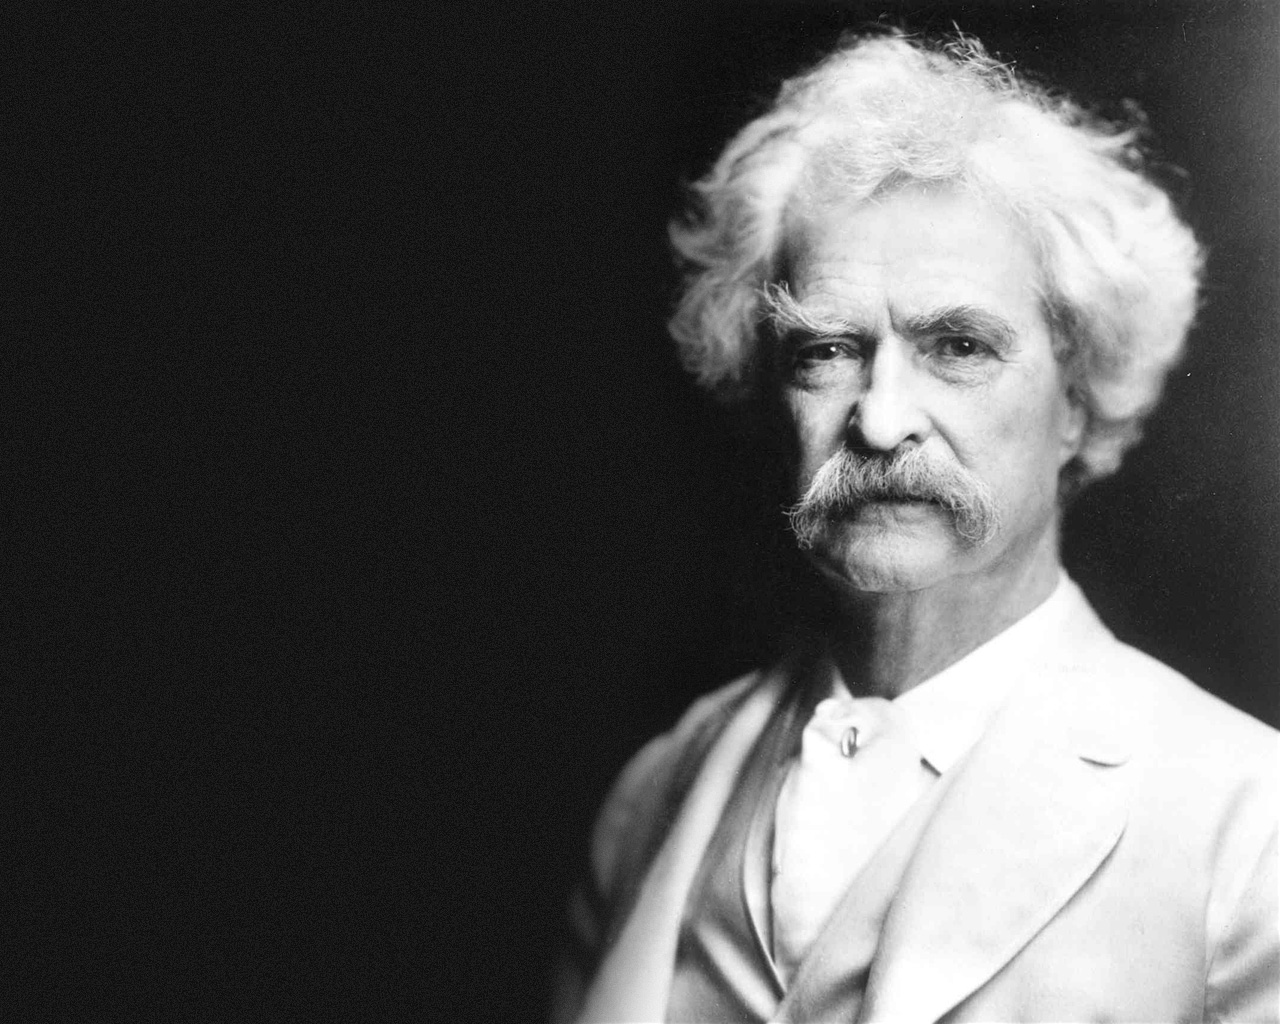
\includegraphics[width=.8\linewidth]{qb/instruction_figures/Mark_Twain}

  \column{.5\linewidth}
  \begin{itemize}

    \item \alert<2>{He} wrote a scathing critique of the Deerslayer.  \alert<2>{His} journey to
  Keokuk in ``Roughing It'' \dots

    \item \alert<2>{Mark Twain} said its virtues were its capitalization and phonetic spelling.

     \item Data is followed by \alert<2>{a white-suited man also
         staying in the hotel}.
       \end{itemize}

\end{columns}

\end{frame}



\begin{frame}
\frametitle{Characters}

\begin{columns}
  \column{.5\linewidth}
  \begin{itemize}


    \item \alert<2>{Mary Johnson} is \alert<2>{the drunkard mother} of \alert<3>{Jimmy} and \alert<4>{the protagonist}

    \item As recorded on the five hundred paper sheets provided by \alert<5>{his} keeper \alert<6>{Bruno Munsterberg}, \alert<5>{this man} eventually takes \alert<7>{Alfred}'s surname

     \item \alert<8>{The protagonist} retrieves a love note from a Bible in a church pew for \alert<9>{Sophia}
       \end{itemize}

  \column{.5\linewidth}
  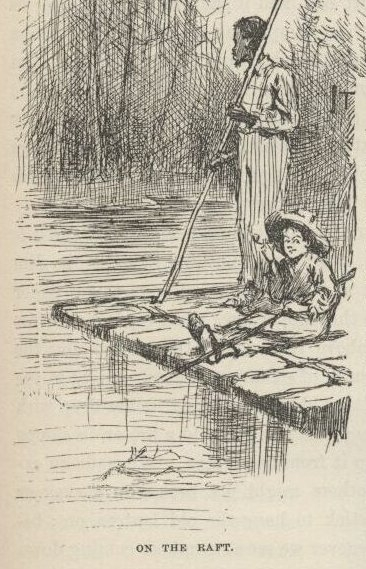
\includegraphics[width=.8\linewidth]{qb/instruction_figures/huck_jim}


\end{columns}

\end{frame}


\begin{frame}
\frametitle{Always Mark the Answer of the Question}


\begin{columns}
  \column{.3\linewidth}
  
\includegraphics[width=1.0\linewidth]{qb/instruction_figures/japan}

  \column{.65\linewidth}

One author from \alert<2>{this country} wrote about a criminal whose climb to heaven is ended when he refuses to let others follow behind him on the title object. \alert<2>{This home to the author of "The Spider's Thread"} had an author write about a group of children confined to a plague-stricken village. Another writer from \alert<2>{this country} wrote a work titled after a mechanical toy about Toru Okada. For 10 points, name \alert<2>{this nation} home to Nip the Buds, Shoot the Kids and The Wind-Up Bird Chronicle authors Kenzaburo Oe and Haruki Murakami.


\end{columns}

\end{frame}


\section{Singletons}

\begin{frame}{Do I have to mark everything?}

\begin{columns}

  \column{.5\linewidth}
\alert<2,10>{His} first publication was \alert<3,10>{a collection of 36 love poems} entitled \alert<3,10>{Chamber Music}. \alert<4,10>{Stephen Hero} was a posthumous publication that contained large portions of \alert<7,10>{another of \alert<2,10>{his} works}, while \alert<5,10>{Humphrey Chimpdon} appears in another work, \alert<6,10>{Finnegan's Wake}. For 10 points, identify \alert<2,10>{this Irish author of \alert<7,10>{A Portrait of the Artist as a Young Man}, \alert<8,10>{Dubliners}, and \alert<9,10>{Ulysses}}.
  \column{.5\linewidth}

\only<2>{
  \begin{block}{Coreference 1}
    \begin{itemize}
      \item His
      \item his
      \item this Irish author of A Portrait of the Artist as a Young Man, Dubliners, and Ulysses
    \end{itemize}
  \end{block}
}

\only<3>{
  \begin{block}{Coreference 2}
    \begin{itemize}
      \item a collection of 36 love poems
      \item Chamber Music
    \end{itemize}
  \end{block}
}


\only<4>{
  \begin{block}{Coreference 3}
    \begin{itemize}
      \item Stephen Hero
    \end{itemize}
  \end{block}
}


\only<5>{
  \begin{block}{Coreference 4}
    \begin{itemize}
      \item Humphrey Chimpdon
    \end{itemize}
  \end{block}
}

\only<6>{
  \begin{block}{Coreference 5}
    \begin{itemize}
      \item Finnegan's Wake
    \end{itemize}
  \end{block}
}


\only<7>{
  \begin{block}{Coreference 6}
    \begin{itemize}
      \item A Portrait of the Artist as a Young Man
      \item another of his works
    \end{itemize}
  \end{block}
}

\only<8>{
  \begin{block}{Coreference 7}
    \begin{itemize}
      \item Dubliners
    \end{itemize}
  \end{block}
}


\only<9>{
  \begin{block}{Coreference 8}
    \begin{itemize}
      \item Ulysses
    \end{itemize}
  \end{block}
}

\end{columns}



\end{frame}

\section{How much to highlight}

\begin{frame}
  \frametitle{How much should I highlight?}

  \begin{itemize}
    \item highlight enough of the text so that it can be grammatically
      replaced by a pronoun
    \item result is grammatical, not sensical
  \end{itemize}

\end{frame}


\begin{frame}{How much should I highlight: Examples}

  \begin{center}
    \replace{For 10 points, name}{this author of No Exit and other French existentialist works}{him}{.}
  \end{center}

\end{frame}


\begin{frame}{How much should I highlight: Examples}

  \begin{center}
    \replace{Beyond Chosen Country and Three Soldiers,}{another of his
      works}{it}{sees Bud Korpening committing suicide, as well as
      John Oglethorpe marrying Ellen Thatcher.}
  \end{center}
\end{frame}


\begin{frame}{How much should I highlight: Prepositions}

  \begin{center}
    \replace{These characters appear in}{a play in which Uncle Ben strikes it rich in Alaska while Happy and Biff are embittered about their father's insistence on living the American Dream}{it}{.}
  \end{center}
\end{frame}

\begin{frame}{How much should I highlight: Prepositions}

  \begin{center}
  
    \replace{For 10 points, name}{this Tennessee Williams play about Blanche Dubois}{it}{.}
  \end{center}
\end{frame}

\begin{frame}{How much should I highlight: Relative Clauses}

  \begin{center}
  
    \replace{Name}{this six-fingered character}{he}{who struggles to get a house in a novel by V. S. Naipaul.}
  \end{center}
\end{frame}

\begin{frame}{How much should I highlight: Relative Clauses}

  \begin{center}
  
    \replace{For ten points, name}{this protagonist}{he}{who cannot evade piloting duty in Joseph Heller's Catch-22.}
  \end{center}
\end{frame}

\begin{frame}{How much should I highlight: Relative Clauses}

  \begin{center}
  
    \replace{For 10 points, identify}{this work}{it}{depicting Umuaro's fall into Christian dominance, a work of Chinua Achebe.}
  \end{center}
\end{frame}

\begin{frame}{This is hard!}

	\begin{itemize}
		\item Talk about issues in the comments fields
		\item Don't need to be perfect
		\item Multiple people will look at each question
		\item This is for {\bf science!}
	
	\end{itemize}

\end{frame}

\section{Other Questions}

\begin{frame}{Hard Question? Need Additional Information?  Skip it!}

One character with this surname is has a vision of the Devil, who mocks him for asserting that all men will unite to take from life all it can give. Another character with this surname studies with Father Zossima. One tells the story of The Grand Inquisitor, while \alert<2>{another member of this family desperately} pursues Grushenka before being falsely convicted for Smerdyakov's murder of Fyodor. For 10 points, Aloysha, Dmitri, and Ivan are all members of what family, which appears in a namesake novel by Fyodor Dostoevsky?

\end{frame}

\begin{frame}{Prizes}

  \begin{itemize}
    \item Vet all users on accuracy
    \item Rank remaining users on number of questions annotated
    \item Top three get prizes (\$20)
    \item Six other random users get prizes (\$15)
    \pause
    \item Think more carefully about early clues in questions
  \end{itemize}

\end{frame}

\begin{frame}{Still have questions?}
  \begin{itemize}
    \item Click on ``contact us'' link on the webpage
  \end{itemize}
\end{frame}


\end{document}